\chapter{1986:Leslie Valiant}
\label{chap:valiant}
\begin{center}
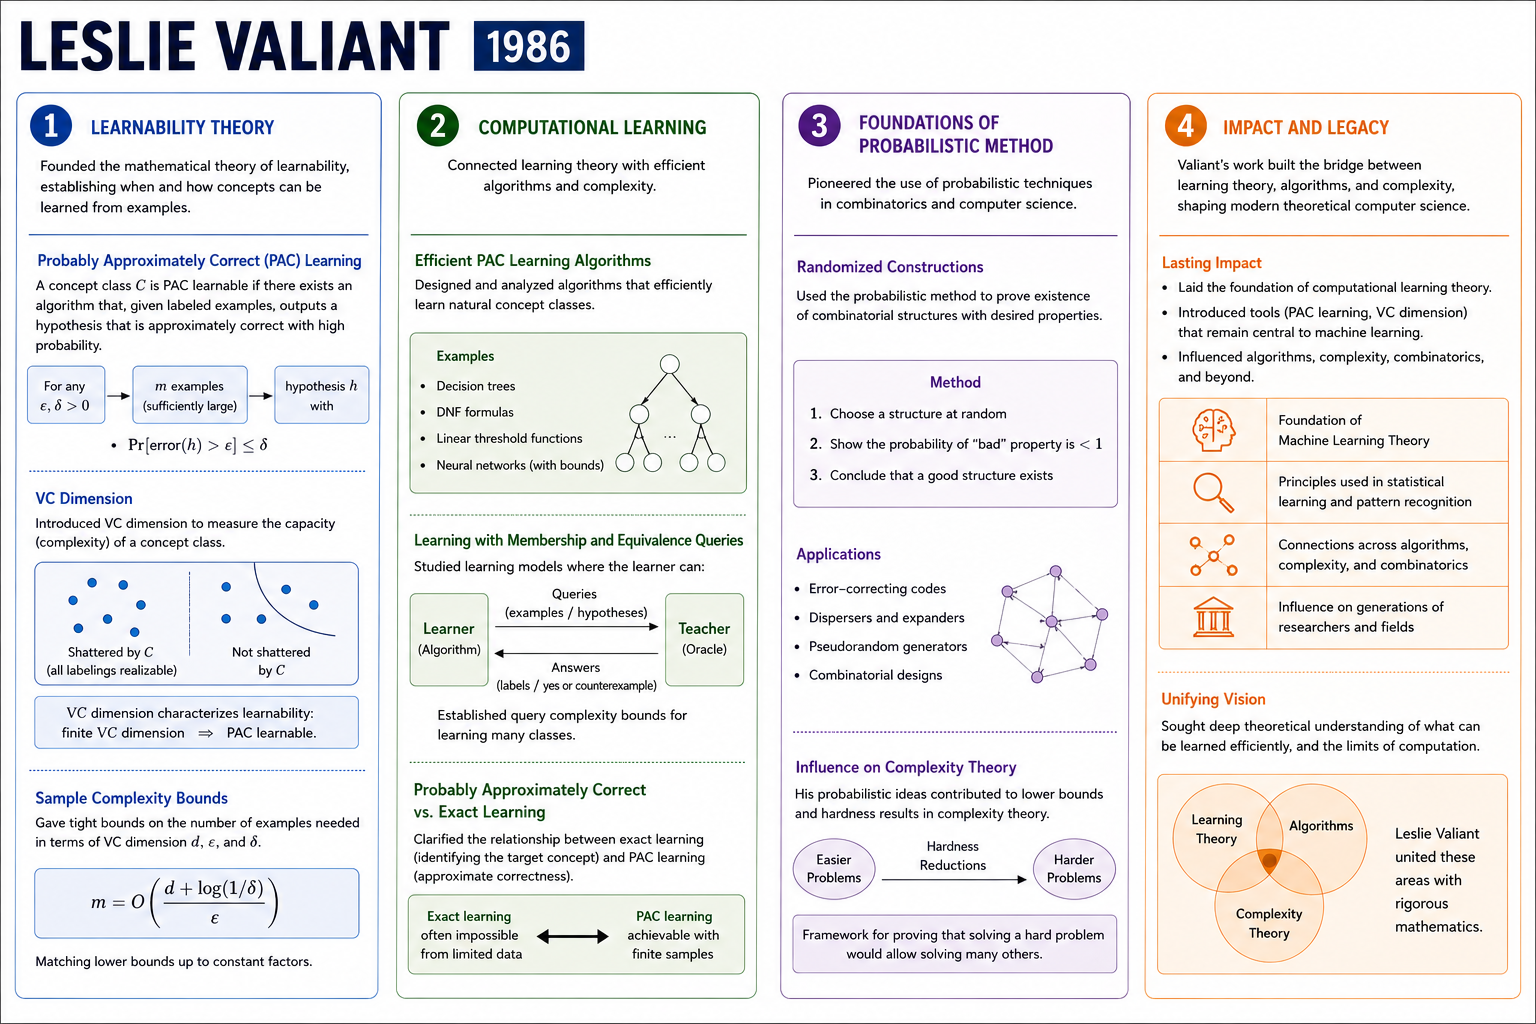
\includegraphics[width=\textwidth]{infographics/abacus2.png}
\end{center}
\longchapterspacing
\index{Valiant, Leslie}
\booknote{The central habit in this chapter is to count the witnesses, not merely to decide that one exists, and to judge a learner by a proven promise about unseen examples rather than by its score on the examples it has already seen.}

\section{An Opening Story: Pairing Up for a Quiz Night}
A quiz club has four members---Alice, Ben, Chen, and Dana---who must form two teams of two for a friendly round. There is one house rule: two members who have already been teammates this month may not pair up again. Only Alice and Ben have played together so far.

The captain asks the obvious question: ``Can we form the two teams at all?'' The answer is one bit: yes. Then the captain asks a quieter question: ``\emph{How many} different ways are there to split the four members into two allowed teams?'' The answer is a number. The full pairings of four people are (Alice,Ben)$+$(Chen,Dana), (Alice,Chen)$+$(Ben,Dana), and (Alice,Dana)$+$(Ben,Chen)---three in total. The first is forbidden, so exactly two survive. The computer had to say \emph{2}, not merely ``yes,'' and it would have had to distinguish 2 from 1 or 3 with equal care. Now grow the club: with 40 members and no restrictions, the number of ways to split into 20 teams is about \(3.2\times10^{23}\), larger than all the stars of the Milky Way, even though ``does any split exist?'' is still answered by one word. The questions look identical but are different computations: one produces a bit, the other a number that can be astronomically large.

This chapter is the mathematics of answering the second kind of question, and of a parallel discovery about learning: the same discipline that separates ``is there one?'' from ``how many are there?'' also separates ``does it fit?'' from ``will it generalize?''

\section{The Problem}
\noindent\textbf{Counting versus deciding.} A \emph{bipartite graph} is a collection of points split into two sides, left \(L\) and right \(R\), with lines (\emph{edges}) joining only left to right. A \emph{matching} is a set of edges in which no two edges share an endpoint; a \emph{perfect matching} uses every point exactly once. Think of the left side as people and the right side as jobs, an edge meaning ``this person can do this job.'' Decision asks whether every person can be assigned a distinct job; counting asks how many complete assignments exist. On a tiny instance---\(L=\{a,b,c\}\), \(R=\{1,2,3\}\), every edge present except \(a\)--\(1\)---the answers are ``yes'' and ``4.''

The same split appears in logic. A \emph{Boolean formula} is a recipe built from variables that are each true or false. The formula \(\varphi=(x\vee y)\wedge(x\vee z)\) over the variables \(x,y,z\) is true for exactly 5 of the 8 possible truth choices. ``Is there any satisfying choice?'' has answer \emph{yes}; ``how many are there?'' has answer \emph{5}.

Why should the second be harder than the first? Because a search can stop the moment it finds one witness, while a count must account for every branch, including those that contain no witness at all. To find a perfect matching you grow an assignment edge by edge, backtracking when a road closes; but backtracking records only ``this branch failed,'' discarding how many completions it contained. The count is a global property of the whole input; each local yes/no answer reveals almost nothing about it.

\noindent\textbf{Learning a rule from examples.} A learner receives examples of the form (features, label). A concrete case: a course records, for each student, the hours studied and whether the student passed. The learner wants a rule---say, a threshold on hours---that predicts the label of the \emph{next} student, who is unseen. Fitting is the easy part: any threshold that agrees with the examples is a candidate. The hard part is a promise about the future: what could justify a statement like ``with 76 examples, any threshold that fits them all misclassifies at most 10 in every 100 new cases, with 95\% confidence''? That claim concerns data never observed, so fitting cannot verify it; it needs a model in which ``generalizes'' has a precise meaning and can be proved.

\section{The World Before}
In the 1970s, Cook and Levin proved that ``does this Boolean formula have a satisfying assignment?'' is the hardest of a whole family of decision problems, and Karp exhibited dozens more with the same status. The central object of the new theory was the \emph{decision problem}: a set of inputs whose answer is yes or no. Complexity was measured by the difficulty of telling yes apart from no, and in the same decade Edmonds showed the matching problem easy for \emph{decision}: polynomial-time algorithms say whether a perfect matching exists and return one if it does.

Because decision was the currency of the field, ``solving'' a problem came to mean finding a single witness, and the folklore reflex for a count was to run the decision procedure repeatedly. This fails even in miniature. For the formula \(\varphi=(x\vee y)\wedge(x\vee z)\), a decision oracle answers ``yes,'' and each time you ask again it returns one witness, say \((1,0,0)\), then another; each answer is a single object. To learn that five exist, you must stop the oracle repeating itself by feeding back what you have already seen---bookkeeping that is enumeration, the counting computation itself. An oracle that answered ``are there at least \(k\)?'' could binary-search the count, but answering ``at least \(k\)?'' is itself a counting question.

Learning was in a similar state, but murkier. The folk model was curve fitting: take a few data points and draw a rule through them. A polynomial can pass through any finite set of points and then go anywhere at all; fitting was never the issue, so nobody could say what was being asked. Statisticians had heuristics---model selection, cross-validation, bias--variance trade-offs---but their claims were not theorems with explicit parameters.

Two conceptual tools were missing. First, a complexity theory for \emph{counting functions} rather than languages, with reductions that preserve the number of witnesses rather than merely the answer to a yes/no question. Second, a mathematical model of learning in which the error, the confidence, the number of examples, and the running time all appear as quantities in a single theorem. Valiant supplied both.

\section{The New Idea}
The first idea: \emph{count the witnesses, and treat the count as a function in its own right.} Suppose \(R(x,y)\) means ``\(y\) is a valid witness for input \(x\)'' with two constraints: each witness has length at most polynomial in the size of \(x\), and checking \(R(x,y)\) takes polynomial time. Define
\[
F_R(x)=\bigl|\{y:\lvert y\rvert\le q(\lvert x\rvert),\,R(x,y)\}\bigr|
\]
for some polynomial \(q\). The family of all such functions is \(\#\mathrm{P}\), read ``sharp P'': the functions that count efficiently checkable, polynomially bounded witnesses. Satisfying assignments, perfect matchings, and schedules all fit this form. The conceptual shift is sharp: \emph{before}, complexity theory studied sets and asked whether an input belongs to one; \emph{the new idea} is that ``how many witnesses does this input have?'' is a different question, whose answer is a possibly enormous integer. Such \emph{parsimonious} reductions---the counting analogue of polynomial-time reductions---must preserve that integer exactly, and they build a hierarchy whose top, \(\#\mathrm{SAT}\) and the \emph{permanent}, is \(\#\mathrm{P}\)-complete.

The permanent is the canonical hard counting function:
\[
\operatorname{perm}(A)=\sum_{\pi\in S_n}\prod_{i=1}^n A_{i,\pi(i)}.
\]
For a zero-one matrix it counts perfect matchings of a bipartite graph. Compare it with the determinant: the same sum, but with a sign \(\operatorname{sgn}(\pi)\) in front of every term. The sign lets elimination cancel most of the sum, which is why determinants run in polynomial time; the permanent has no cancellation, and Valiant proved it \(\#\mathrm{P}\)-complete. A single bit of information---which sign to attach---separates easy from believed-hard.

The second idea, for learning, is an explicit contract rather than a new complexity class. In the \emph{Probably Approximately Correct} (PAC) model, examples are drawn independently from an unknown distribution \(D\). The learner picks a hypothesis \(h\) from a class \(H\), and the guarantee is: with probability at least \(1-\delta\) over the sample, the probability that \(h\) errs on a fresh draw is at most \(\varepsilon\). Both the sample size \(m\) and the running time are charged. \emph{Before}, people thought learning was fitting; \emph{the new idea} is that learning is a theorem of the form ``with \(m\) samples, whatever hypothesis the algorithm chooses is good,'' where the key move is to prove the guarantee for \emph{all} hypotheses in \(H\) simultaneously---because the chosen one depends on the sample, it cannot be certified after the fact.

\section{How It Works: Worked Examples}
\subsection{Counting perfect matchings, line by line}
Take \(L=\{a,b,c\}\), \(R=\{1,2,3\}\), and every edge except \(a\)--\(1\). A perfect matching pairs each left point with a distinct right point, so it is exactly a permutation of \(\{1,2,3\}\) with \(a\) not paired with 1. Enumerate:

\begin{center}
\begin{tabular}{lccc}
\toprule
matching & assignment & uses \(a\)--1? & allowed? \\
\midrule
\(a\)--1, \(b\)--2, \(c\)--3 & 123 & yes & no \\
\(a\)--1, \(b\)--3, \(c\)--2 & 132 & yes & no \\
\(a\)--2, \(b\)--1, \(c\)--3 & 213 & no & yes \\
\(a\)--2, \(b\)--3, \(c\)--1 & 231 & no & yes \\
\(a\)--3, \(b\)--1, \(c\)--2 & 312 & no & yes \\
\(a\)--3, \(b\)--2, \(c\)--1 & 321 & no & yes \\
\bottomrule
\end{tabular}
\end{center}

Of the \(6=3!\) permutations, the two using the missing edge are discarded, leaving 4. The decision answer is ``yes,'' one bit; the count must tell this graph, with its 4 perfect matchings, apart from a graph with 1, 2, or 6. A decision algorithm returns a single matching and stops; to reach the number 4 it would have to find all four without repeating one---maintaining the list it has already produced, the counting work in disguise.

\subsection{The satisfying assignments of a tiny formula}
For \(\varphi=(x\vee y)\wedge(x\vee z)\), test all 8 assignments:

\begin{center}
\begin{tabular}{ccccc}
\toprule
\(x\) & \(y\) & \(z\) & \((x\vee y)\) & \((x\vee y)\wedge(x\vee z)\) \\
\midrule
0 & 0 & 0 & 0 & 0 \\
0 & 0 & 1 & 0 & 0 \\
0 & 1 & 0 & 0 & 0 \\
0 & 1 & 1 & 1 & 1 \\
1 & 0 & 0 & 1 & 1 \\
1 & 0 & 1 & 1 & 1 \\
1 & 1 & 0 & 1 & 1 \\
1 & 1 & 1 & 1 & 1 \\
\bottomrule
\end{tabular}
\end{center}

The count is 5. A more instructive way to see it: split on \(x\). If \(x=1\), both clauses are already satisfied and \(y,z\) are free, giving \(2\cdot2=4\) assignments. If \(x=0\), the clauses reduce to \(y=1\) and \(z=1\), giving exactly one. Total: \(4+1=5\). A decision search walks down one branch and stops; only an algorithm that keeps both branches and adds their counts returns 5.

\subsection{Learning a threshold, with a number attached}
Suppose the unknown rule is ``pass iff hours \(\ge 3\).'' Four samples arrive: hours 1 and 2 fail; hours 3.5 and 5 pass. The learner's class is thresholds \(x\ge t\); a natural choice, \(t=2.5\), sits just past the largest negative example and fits the sample, but so does \(t=3.1\). The two hypotheses differ exactly in the strip between 2.5 and 3.1, which the sample never shows. In general, a consistent threshold can err only inside the \emph{gap} between the largest negative and the smallest positive sample point, and its risk is at most the probability mass of that gap.

Now suppose the learner restricts itself to \(N=100\) candidate thresholds, so the class is finite. Fix one candidate whose true error is at least \(\varepsilon=0.1\). The probability that it makes no mistake on \(m\) random samples is at most
\[
(1-\varepsilon)^m\le e^{-\varepsilon m}.
\]
By the union bound, the probability that \emph{some} candidate is bad and yet fits the sample is at most \(100\,e^{-\varepsilon m}\). Forcing this below \(\delta=0.05\) gives
\[
m\ge\frac{1}{\varepsilon}\ln\frac{N}{\delta}=10\ln 2000\approx 76.
\]
So about 76 samples suffice: with probability at least 95\%, every candidate threshold that fits the sample has true error at most 10\%, and therefore so does the one the learner chose. The bound is \emph{uniform}---proved for all 100 candidates before the sample is drawn---so it covers whichever hypothesis the data selects; a non-uniform argument would be circular, because the chosen hypothesis is a random function of the very sample used to evaluate it.

\section{The Mathematics in Brief}
A function \(F\) belongs to \(\#\mathrm{P}\) when \(F(x)=\abs{\{y:\lvert y\rvert\le q(\lvert x\rvert),\,R(x,y)\}}\) for a polynomial \(q\) and a relation \(R\) checkable in polynomial time: the value counts \emph{witnesses}, and both the witness length and the checking time are polynomially bounded. A \emph{parsimonious reduction} maps instances of one counting problem to instances of another so that the number of witnesses is preserved exactly; \(\#\mathrm{SAT}\) and the permanent are \(\#\mathrm{P}\)-complete. Why is the permanent \(\#\mathrm{P}\)-complete? Valiant reduced \(\#\mathrm{SAT}\) to the permanent by way of \emph{cycle covers}. The permanent of the adjacency matrix of a directed graph with edge weights \(0,\pm1\) sums, over all ways to cover the vertices with disjoint directed cycles, the product of the weights on those cycles---a sum of exactly the right shape to simulate counting. Each Boolean variable becomes a small gadget with exactly two surviving local configurations, recording its truth value; each clause becomes a gadget whose cycles survive precisely for the assignments that satisfy it. The graph is built so that the only nonzero cycle covers correspond one-for-one with satisfying assignments, making the permanent equal the count. Hence a polynomial-time permanent algorithm would compute \(\#\mathrm{SAT}\), and hardness has teeth: by Cook--Levin it would put satisfiability (ask whether the count is zero) in polynomial time, and Toda's theorem extends the reach of a single counting computation beyond the whole polynomial hierarchy. Yet the difficulty is really about magnitude, not about the objects: the permanent and determinant are identical except for signs, and since \(-1\equiv 1\pmod 2\), the parity of the number of perfect matchings is computable in polynomial time as a determinant. Counting mod 2 is easy; counting exactly is believed impossible.

The PAC guarantee has the structure
\[
\text{true error}(h)\;\le\;\text{training error}(h)+\text{complexity penalty}.
\]
For a finite class of size \(N\), the penalty carries a \(\ln N\) term; the bound \(m\ge\frac1\varepsilon\ln\frac N\delta\) follows from the union bound---for a fixed hypothesis with true error at least \(\varepsilon\), the chance it looks perfect on \(m\) samples is at most \(e^{-\varepsilon m}\), multiply by the number of hypotheses, and solve for \(m\). The empirical picture transfers to new data \emph{simultaneously for the whole class}, which makes it valid for a hypothesis chosen by looking at the sample.

\section{Limits and Modern Views}
Exact counting of witnesses is believed impossible in polynomial time, so modern work asks what can be saved. One line, \emph{approximate counting}, accepts a multiplicative estimate and uses Markov chains: design a random walk whose stationary distribution weights each matching correctly, let it mix, and average an observable over the walk. This replaces the impossible exact count with a sampler, but only when the chain mixes fast. The permanent admits a fully polynomial-time randomized approximation scheme for nonnegative matrices (Jerrum, Sinclair, and Vigoda), and the subject is haunted by \emph{bottlenecks}: a chain whose state space is two dense regions joined by a narrow corridor takes exponentially long to cross it. Sampling, counting, and the geometry of the state space are one theorem.

The PAC model has aged in two ways. It is a worst-case guarantee over distributions: it holds for any \(D\), which is honest but demands more than practice needs, so modern learning theory adds structure---VC dimension replaces \(\ln N\) for infinite classes, noise and robust estimation change the loss, privacy budgets a new resource. And PAC is only the \emph{statistical} clause of learning. A hypothesis class can be statistically learnable while no efficient algorithm finds the hypothesis, and a rule that generalizes under \(D\) can fail when the future differs from the past. Valiant's insistence that error, confidence, samples, and running time be accounted together remains the frame in which all these refinements are stated \cite{valiant-counting,valiant-learning}.

\section{Exercises and Self-Study Guide}
\begin{enumerate}[label=\textbf{E\arabic*.}]
\item Verify by listing: how many assignments of \((x,y,z)\in\{0,1\}^3\) satisfy \((x\vee y)\wedge(y\vee z)\wedge(z\vee x)\)?
\hint{Only four of the eight assignments are excluded. Group the exclusions by which pair of variables is both 0.}
\item In the worked matching graph, remove a second edge, \(b\)--\(2\), in addition to \(a\)--\(1\). Count the perfect matchings using inclusion--exclusion.
\hint{Start from \(3!=6\). The 2 matchings using \(a\)--\(1\) and the 2 using \(b\)--\(2\) overlap in the 1 matching using both, so \(6-2-2+1=3\).}
\item Give a counting problem whose decision version is easy but whose count is believed hard, and explain why calling the decision algorithm repeatedly does not help.
\hint{2-satisfiability is solvable in polynomial time, yet counting its satisfying assignments is \(\#\mathrm{P}\)-complete.}
\item Derive the union-bound sample size \(m\ge\frac1\varepsilon\ln\frac N\delta\) from scratch, and re-check the number 76.
\hint{Fix one hypothesis with true error at least \(\varepsilon\); bound the chance that it is clean on \(m\) samples by \(e^{-\varepsilon m}\); union over all \(N\) and solve for \(m\).}
\item Give two thresholds that agree on the sample \(\{1,2,3.5,5\}\) but disagree on an unseen region, and state what extra information would distinguish them.
\hint{Any \(t\in(2,3.5]\) is consistent with the sample; two such thresholds differ on the strip between them, where the risk lives.}
\item Describe a Markov chain whose states are the perfect matchings of a small bipartite graph, and draw a graph for which the chain has a clear bottleneck.
\hint{Let a step move to a new matching by toggling one or two edges, with proposal probabilities chosen to keep the chain symmetric; a bottleneck is two large families of matchings joined by very few intermediate matchings.}
\item Take the claim ``a learner trained on these examples will generalize.'' Separate it into a statistical clause, a computational clause, and a robustness clause, and say which one the PAC theorem actually proves.
\hint{The theorem proves the statistical clause under the assumption that samples are independent draws from a fixed distribution; the computational clause concerns the algorithm's running time, and the robustness clause concerns what happens if the future distribution differs.}
\end{enumerate}

\booknote{A final exercise in judgment: whenever someone hands you a number that claims to describe how many, or a learner that claims to have generalized, ask which parts of the claim are theorems, which parts are assumptions, and which parts are hope---and state what data, or what reduction, would have to exist to convert each hope into a theorem.}
\clearpage
